% !TEX spellcheck = en-US

\chapter{Locality Sensitive Hashing}
	
	The goal of hashing techniques is to reduce a big ``object" to a small ``signature" or ``fingerprint".\\
	In general, what happens in locality sensitive hashing (or LSH) is to have some notion of similarity, and then define a ``scheme" which computes it. The process of creating a scheme usually involves some sort of preprocessing step, and a function family which, by choosing one or another function according a probability distribution, statistically classifies the objects in the same way as the similarity function does.\\
	The bottom line of LSH schemes is: similar objects hash to similar values (this is ``\textit{locality}").
	
	Here are some common similarities:
	
    \begin{defn}[Jaccard similarity]
        Given two sets of objects A and B, their Jaccard similarity is defined as follows:
        \begin{equation}
        \jaccsim(A, B) = \frac{|A\cap B|}{|A\cup B|}
        \end{equation}
    \end{defn}
	
    \begin{defn}[Hamming similarity]
        Given two sets of objects A and B taken from a universal set U, their Hamming similarity is defined as follows:
        \begin{equation}
        \hammsim(A, B) = \frac{|A\cap B| + \abs{\overline{A\cup B}}}{|U|}
        \end{equation}
    \end{defn}

    \begin{obs}
        Generally, the Jaccard similarity is more used then the Hamming similarity, because usually we have to compare sets whose size is much smaller than the size of the universe set $U$, this, using $\hammsim$, we would obtain a high similarity because of the big size of $\overline{A\cup B}$.
    \end{obs}


\section{A case study: Web-page indexing}\label{sec:web-page-indexing}
	
	A search engine crawls periodically the whole Internet and stores valuable information in its own index for search optimization purposes.
	
    \begin{obs}
        Some kinds of documents, that are very similar to each other, are stored sparsely through the net; to save storage space, only one of a kind of document's info is stored in the index, whereas all others are linked to the first one, because of their similarity.
    \end{obs}
	
	To find a useful hashing scheme, A. Broder came up with an idea, and he succeeded in reducing the storage space needed by Altavista by a factor of 10.
    
	First off, let us fix some definitions:
	\begin{itemize}
	\item $U$: the set of all words, i.e. the English vocabulary
	\item $U^*$: the set of all strings composed of English words
	\end{itemize}
	
	The starting point is to treat web pages as strings:
	
	$T_1:$ \textit{``The black board is black''}
	
	$T_2:$ \textit{``The white board is white''}
	
	Then, let $distinct(T)$ return the set of distinct words appearing in a string (ref. \href{https://en.wikipedia.org/wiki/Bag-of-words_model}{Bag of Words model}), and let $A:=distinct(T_1),\ B:=distinct(T_2)$.
    
    \begin{figure}[h!]
        \centering
        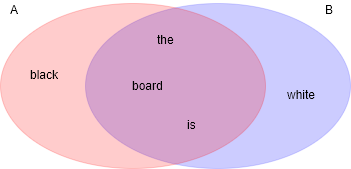
\includegraphics[scale=0.7]{bow_venn}
        \caption{Venn diagram with the BoW representation of $T_1$ and $T_2$.}
        \label{fig:bow_venn}
    \end{figure}
	
	So for example, by using the Jaccard similarity:
    
    \begin{equation}
    \jaccsim(A, B)= \frac{3}{5}
    \end{equation}
	
	Over a half: they look close. If we used the Hamming distance instead, we would (almost always) get a number very close to 1, because we're using a minuscule part of the universe set (in our case, the English dictionary), thus (almost) all words are absent from the sets.
	
	Now, our objective is to construct a scheme over web-pages that implement the Jaccard similarity.\\
	Our pre-processing step: Choose a permutation (or total ordering) $\pi \in \order(A \cup B)$ \uar. To construct said order is a simple task, as we can see with the following algorithm.
	
	Algorithm for sampling a $\uar$ permutation $\pi$ of $[n]$, where $[n]$ is a numeric representation of $U$, and using it to compute the hash of $A$:
	\begin{lstlisting}[caption={min hash or shingles algorithm},label={lst:min_hash}]
MinHash($A$):
     // preprocessing
     $S$ := $[n]$
     $\pi$ := empty sequence
     while $S \neq \emptyset$:
         pick $i \in S \ \uar$
         append $i$ to $\pi$
         remove $i$ from $S$
     end
     // computing hash
     $h_\pi(A)$ := minimum element of A, accordig to $\pi$
     return $h_\pi(A)$
	\end{lstlisting}
	
    \begin{proof}[Proof of uniform choice of $\pi$]
        \begin{align*}
        \Pr{X = \pi} &= \frac{1}{|S|}\cdot\frac{1}{|S|-1}\cdot\dots\cdot 1\\
        &= \frac{1}{|S|!} \Rightarrow X \in \unifdist(\permut(A \cup B))
        \end{align*}
    \end{proof}
	
	So, from $\pi$, we obtained the following definition:
    \begin{defn}[Hashing function]
        \begin{equation}
        h_\pi \in \mathcal{P}(U) \to U : h_\pi(A) = min_\pi(A)
        \end{equation}
    \end{defn}
	
	In other words, we take the ``minimum'' in A according to the ordering specified by $\pi$.
    
    \begin{obs}
        A simple but useful observation would be:
        \begin{equation}
        \forall A \subseteq U \Rightarrow h_\pi(A) \in A
        \end{equation}
    \end{obs}
	
	\begin{ex}
       	\begin{equation*}
            \pi = (black, the, is, white, board) \wedge A = \{the, black, board, is\} \Rightarrow h_\pi(A) = black
        \end{equation*}
    \end{ex}
	
	Thus, we say that $A$ is similar to $B$ iff $h_\pi(A)=h_\pi(B)$.\\
	Recall that $A$ and $B$ are fixed, $\pi$ is the focus of this definition. What can be said about $\Pr{h_\pi(A)=h_\pi(B)}$? Looking at a corresponding Venn diagram [\ref{fig:bow_venn}]:
	\begin{itemize}
	\item $A \cap B = \emptyset \Rightarrow \Pr{h_p(A)=h_p(B)} = 0$; they have no words in common, so their hashes must be different, independently of the chosen order;
	\item $A = B \Rightarrow \Pr{h_p(A)=h_p(B)} = 1$; this time, all words are in common, so their hashes must coincide, again, independently of the chosen order;
	\item Otherwise, since $\pi$ is chosen \uar, the probability that the hashes are equal has the same meaning of the probability of finding the lowest element of A and B in the intersection with respect of the union (and not in $U$ as a whole, as our previous observation suggests), which is the Jaccard similarity of $A$ and $B$ by its very definition:
	\begin{align*}
		\Pr{h_\pi(A)=h_\pi(B)} &= \frac{\Pr{\min(A) \in A \cap B \wedge \min(B) \in A \cap B}}{\Pr{\min(A) \in A \cup B \wedge \min(B) \in A \cup B}}\\
		&= \frac{\abs{A \cap B}}{\abs{A \cup B}} = \jaccsim(A, B).
	\end{align*}
	\end{itemize}
	
	\textit{Possible question about third point}: Why not respect to the universal set? because $A$ and $B$ will have hashes which, as we observed earlier, do not live outside the union: the union between $A$ and $B$ is our true set of outcomes when hashing either $A$ or $B$.
	
	Now, if $h_\pi$ is evaluated only once over a given permutation, only a binary response can be obtained. In order to obtain the probability value without resorting to compute unions and intersections, we can repeat evaluation over different permutations; this can be regulated by the \textbf{Chernoff-Hoeffding bound}:
	
	Let $A, B \subseteq U$, and $X_{1 \dots n} \in \coin(p)$ \iid, with $\Pr{X_i=1}=p$ and $\Pr{X_i=0}=1-p$, with each $X_i$ defined over a distinct element of $\Pi \subseteq \mathcal{P}erm(U)$, such that $X_i \mapsto 1 \Leftrightarrow A \sim_{\pi_i} B, 0\ otherwise$, then:
	\begin{equation} \label{chernoff_hoeffding}
	\Pr{\abs{avg_{i=1}^{n}(X_i - p)}\geq\varepsilon} \leq 2e^{-n\varepsilon^2}
	\end{equation}
	In other words, the difference between the average of the $X_i$ (i.e., the average of the empirically observed results) and their exact probability is greater then $\varepsilon$ only with a very small probability.
	
	So, how many trials (evaluations, observations) are needed to have a good estimate of the similarity? That is, what is a good value for $n$?\\
	Let $
		X_i=\begin{cases}
		1 & \text{if}\ h_{\pi_i}(A)=h_{\pi_i}(B)\\
		0 & \text{otherwise}\\
		\end{cases} $
	and $\Pr{X_i=1} = \jaccsim(A,B)=p$; we can apply the Chernoff bound on $X_i$ to compute our $n$.\\
	If our database has $m$ pages (sets) to store, we can chose $n = \frac{\lg{\frac{2m}{\delta}}}{\varepsilon^2}$ to get a high probability of making zero errors; $\delta$ and $\varepsilon$ are parameters we can set to adjust the size of $n$: even if the bound gives us a high probability for a quite small $n$, we can choose an even smaller $n$ if we can accept big errors for very few pages.
	
	We can now observe that the min hash algorithm [\ref{lst:min_hash}] is efficient: instead of comparing two entire pages, it only compares $n$ integers.

\section{A case study: Comparing DNAs}
	In the previous case study, we considered small subsets of the universe set: each web page has only few words with respect to the whole English language.\\
	However, there are cases in which the overlays between two subsets are often relevant, for example, if we want to compare the DNA of two people.\\
	In such cases, the Hamming similarity is preferable (more significant) to the Jaccart similarity.
	
	We can describe two DNA sequences $A$ and $B$ as two arrays of size $n$, in which each position corresponds to a certain component of the DNA, and contains a 1 if that component is present in that sequence and a 0 if it's absent.
	\begin{align*}
		\hammsim(A,B) &=
		\frac{\abs{A \cap B} + \overline{\abs{A \cup B}}}{n}\\
		&= \frac{\text{number of common } 1s + \text{number of common } 0s}{n}
	\end{align*}

	To get our hash function we pick an index $i\in[n]$ \uar, and we define\\
	$ h_i(A)=\begin{cases}
		1 & \text{if}\ i \in A\\
		0 & \text{otherwise}\\
	\end{cases} $. \label{hamming_hash}
	
	\begin{ex}
        We have two DNA sequences $A$ and $B$ such that $A:=$
        \begin{tabular}{|c|c|c|c|c|c|c|c|}
            \hline
            0 & 0 & 0 & 1 & 1 & 0 & 0 & 1 \\
            \hline
        \end{tabular},
        $B:=$
        \begin{tabular}{|c|c|c|c|c|c|c|c|}
            \hline
            0 & 1 & 1 & 0 & 0 & 1 & 1 & 1 \\
            \hline
        \end{tabular} and $n:=8$, so we can write $A$ and $B$ as $A=\{4,5,8\},\\ B=\{2,3,6,7,8\}$ using the positions with a $1$ inside (starting from $1$).\\
        If we randomly choose $i=8$, we obtain $h_i(A)=h_i(B)=1$, so we can conclude that $A$ and $B$ are similar.
    \end{ex}
    
	
	Now we can see that the probability that two hashes are equal is the Hamming similarity:
	\begin{align*}
		\Pr{h_i(A)=h_i(B)} &= \frac{\Pr{A[i]=B[i]}}{n} \\
		&= \frac{\Pr{(A[i] \text{ and } B[i] \text{ are both } 1) \vee (A[i] \text{ and } B[i] \text{ are both } 0 )}}{n} \\
		&= \frac{\abs{A \cap B} + \overline{\abs{A \cup B}}}{n} = \hammsim(A,B)
	\end{align*}
	
	It's possible to obtain a good estimate of the similarity by repeating the test an appropriate number of time, given by the Chernoff Bound.

\section{LSH formalization}

    First let us focus around the hash function as an object: its true purpose in a scheme is to classify objects based on how much they ``look like'', whatever this means in the chosen similarity's terms. Therefore, in our theoretical analysis, the codomain of a hash function is not that important; what is important is how the function partitions its own domain, $U$. In a sense, we're interested only in the partitions of $U$ themselves, not in the functions that generate them.
    
	Why have we dealt with functions back then? Moving from a purely mathematical perspective to a more computational one, what is usually done for measuring similarities is sampling some object's characteristics, and observe how ``distant'', or else ``similar'' they are. This is done by means of some program; and programs are (oh so) easily associated with functions. The computational approach gives a more intuitive vision of the problem we're confronting ourselves with.
    
    Still, what could happen, is to have a couple of functions that map values into wildly different codomains, but partition $U$ in exactly the same way! And in our journey, we're just interested in classifying objects; so these kind of ``duplicate'' functions are, well, useless (unless we delve in complexity studies, but that's out of our scope).
    
	So, let us reform the foundations by taking as our core object a universe partition, instead of a universe-domained hash function. First, though, we need to formalize what a similarity is, and to get to a good definition, we have to carefully select them from their space $U^2 \to [0, 1]$. It should be noted that the codomain might very well be $\real$ itself, but to get some bearings we'll treat an image of 1 as a complete equivalence between two objects, and 0 for complete difference, with the interval expressing the degree of similarity.
	
	Let $U$ be a set, and $S \in U^2 \to [0, 1]$ a symmetric function; then $S$ is called a \textbf{similarity} over $U$.
	% TODO Still incomplete, need the trineq on 1-S
	
	Tidbit: Let $f \in A^n \to B$, then f is \textbf{symmetric} iff \textit{argument order does not change the image}. % COMMUTATIVITY? Kinda...
	
	\ex \begin{align*}
		& U=2^{[n]}=\left\lbrace A | A \subseteq [n] \right\rbrace \\
		& S=\jaccsim \\
		& S\left( \left\lbrace 1,2 \right\rbrace , \left\lbrace 2,3 \right\rbrace \right) =\frac{1}{3}
	\end{align*}
	
	% A scheme-similarity defines a partition over U
	A \textbf{LSH scheme} over $U$ is a probability distribution over the partitions of $U$.
	
	\ex We can apply the min-hash scheme [\ref{lst:min_hash}] to the Jaccard Similarity. With $U=[3]$ and $\pi = 1<2<3$, the function maps each subset of $U$ to a hash as follows:
	\begin{align*}
		\emptyset &\mapsto \perp \text{(the hash of the empy set is a special symbol)} \\
		\{1\}, \{2,1\}, \{1,3\}, \{1,2,3\} &\mapsto 1 \text{ (all sets containing 1 have hash 1)} \\
		\{2\}, \{2,3\} &\mapsto 2 \text{ (all remaining sets containing 2 have hash 2)} \\
		\{3\} &\mapsto 3 \text{ (all remaining sets containing 3 have hash 3)}
	\end{align*}
	thus defining 4 partitions over $U$.
	
	\ex Similarly, we can apply the function based on the Hamming Similarity we saw in [\ref{hamming_hash}] to the same set $U=[3]$ and see we get new partitions. We choose $i = 2$ \uar, the function maps each subset of $U$ to a hash as follows:
	\begin{align*}
	\{2\}, \{2.1\}, \{2,3\}, \{1,2,3\} &\mapsto 1 \text{ (all sets containing $i$ have hash 1)} \\
	\emptyset, \{1\}, \{3\}, \{1,3\} &\mapsto 0 \text{ (all remaining sets have hash 0)}
	\end{align*}
	thus defining 2 partitions over $U$.
	
	Let's make some other considerations about what we have just seen.
	
	%%%%%%%%%%%%%%%%%%%%
	
	% Intuitive: a hash function's purpose is to map arguments that are very similar to the same value
	
	% Hash function: $h \in U \to (*)$ such that the domain's representation is 'sensibly smaller' than U (h is NOT injective by this intuition - not true, injective functions are used as hash functions in pathological cases...)
	
	% Insight: A hash function seems to complicate definitions more than a simple equivalence relation, but it models programs/algorithms more effectively, which is our focus here
	
	\obs Given a similarity $\phi$, a LSH scheme is a family of hash functions $H$, coupled with a probability distribution $D$ over $H$ such that, chosen a function $h$ from the family $H$ according to $D$, $h$ satisfies the property $\Pr{h(a)=h(b)} = \phi(a,b) \forall a,b \in U$. \\
	In other words, let $S \in U^2 \to [0, 1]$ be a similarity, and H be a RV over a family of hash functions over U, then H is a LSH scheme iff $\Pr{H(a)=H(b)} = S(a,b) \forall a,b in U$
	
	% Brainlamp: I can extend the domain of H to the whole hashfunction class by setting the outsiders' probability to 0...
	%%%%%%%%%%%%%%%%%%%%%%%%%%%%%%%%%%%%
	
	
	% Note: some partitions will never be a result of a hash function % Hah, not so sure...
	
	% Other note: some form of transitivity must hold. (So yeah, we're dealing with an equivalence relation in the guise of a function with arbitrary codomain)
	
	%\
	
	% INSIGHT
	\obs Preprocess and hash function (aka a scheme) determine the similarity function (most people attempt to do the reverse)
	
	% MAJOR INSIGHT:
	\obs In the previous webpage example [\ref{sec:web-page-indexing}], we're not dealing with a single hashing function, but with a family of functions each built with its own word permutation: the scheme distributes over the permutations of the union!
	% Now, do all permutations induce unique partitions?
	
	%\
	
	% Wrapup:
	Before going on, let's recap what we have discussed so far: \\
	A LSH scheme for a similarity $S$ is a prob. dist. over $U$'s partitions such that 
	\begin{equation}
		\forall A, B \in  U \Rightarrow \Pr{A\sim_p B}_p = S(A, B) = \Pr{h(A)=h(B)}_h
	\end{equation}
	where $p$ is a partitioning of $U$ and $\sim_p$ means $A$ and $B$ are in the same partition.
	
	Another possible definition: Given $s \in U^2 \to [0,1]$ a similarity, then we define $X$ to be a LSH scheme for $s$ as the following:
	\begin{equation}
	X \in \probdist(\powerset(U)) : \forall A, B \in U \implies \expect(A\sim_X B) = S(A, B)
	\end{equation}
	
	\textit{Challenge}: Can we find a LSH scheme for an arbitrary S function? NO
	
	\ex \label{ex:transitivity} Given a universe set $U = \{a, b, c\}$ and a similarity function $S$ s. t.	$S \in U^2 \rightarrow [0, 1] : S(a, b) \mapsto 1, S(b, c) \mapsto 1, S(a, c) \mapsto 0$ we don't have an LSH, since we're violating transitivity:
	Translating into probabilities and using equality's transitivity, we obtain: $\Pr{h(a), h(c)}=1$, which contradicts the third mapping.
	